\chapter{Лабораторная работа №2. Реализация ШИМ-контроллера скорости вентилятора}

ШИМ или PWM (широтно-импульсная модуляция, по-английски pulse-width modulation) – это
способ управления подачей мощности к нагрузке. Управление заключается в изменении
длительности импульса при постоянной частоте следования импульсов, то есть при использовании метода широтно-импульсной модуляции, 
частота сигнала и амплитуда остаются постоянными. 
Самым важным параметром сигнала ШИМ является коэффициент заполнения, 
который можно определить по следующей формуле:

\begin{equation}	
	D =  \tau/T
\end{equation}

где \(T\)— период импульсов, \(\tau\)  — длительность импульса, \(D\) — коэффициент заполнения. На рисунках ~\ref{fig:pwm_30}, ~\ref{fig:pwm_70}, ~\ref{fig:pwm_90} представлен ШИМ-сигнал
с различными коэффициентами заполнения.

\begin{figure}[h]
    \centering
    \noindent
    \begin{tikzpicture}
        \begin{axis}
            [
            RCS Plot,
            title={},
            height=0.3\textwidth,
            xlabel={Время, мкс},
            ylabel={Амплитуда, В},
            legend pos = south east
            ]
            \addplot table {Synopsis/data/third-party/pwm_30.dat};
            \addlegendentry{D = 30};
        \end{axis}
    \end{tikzpicture}
    \caption{ШИМ-сигнал с коэффициентом заполнения D = 30}
    \label{fig:pwm_30}
\end{figure}

\begin{figure}[h]
    \centering
    \noindent
    \begin{tikzpicture}
        \begin{axis}
            [
            RCS Plot,
            title={},
            height=0.3\textwidth,
            xlabel={Время, мкс},
            ylabel={Амплитуда, В},
            legend pos = south east
            ]
            \addplot table {Synopsis/data/third-party/pwm_70.dat};
            \addlegendentry{D = 70};
        \end{axis}
    \end{tikzpicture}
    \caption{ШИМ-сигнал с коэффициентом заполнения D = 70}
    \label{fig:pwm_70}
\end{figure}

\begin{figure}[h]
    \centering
    \noindent
    \begin{tikzpicture}
        \begin{axis}
            [
            RCS Plot,
            title={},
            height=0.3\textwidth,
            xlabel={Время, мкс},
            ylabel={Амплитуда, В},
            legend pos = south east
            ]
            \addplot table {Synopsis/data/third-party/pwm_90.dat};
            \addlegendentry{D = 90};
        \end{axis}
    \end{tikzpicture}
    \caption{ШИМ-сигнал с коэффициентом заполнения D = 90}
    \label{fig:pwm_90}
\end{figure}

В качестве коммутационных элементов применяются биполярные и полевые транзисторы,
работающие в ключевом режиме. То есть, часть периода транзистор полностью открыт, 
а часть периода — полностью закрыт. При этом в замкнутом состоянии 
сопротивление транзистора как ключа очень невелико, и падение на нем напряжения приближается к нулю.

После рассмотрения принципов широтно-импульсной модуляции передём к разработке модуля, реализующего данную функцию.
Прежде всего создадим модуль верхнего уровня и рассмотрим вопрос о изменении входной тактовой частоты сигнала равной 200 МГц. .
Для понижение тактовой частоты до 25 МГц используем примитив MMCM(Mixed-Mode Clock Manager). Данный примтив позволяет генерировать до семи различных частот, с различными коэффициентоми заполнения, с различными фазами. Также он может работать в режиме фильтра дрожжания тактового сигнала.
Рассмотрим подробнее параметризацию и принцип работы примитива MMCM, опираясь на документ 7 Series FPGAs Clocking Resources User Guide (UG472). Структурная схема примитива представлена на рисунке ~\ref{MMCM2_BASE}. 

На структурной схемы представлены:

\begin{enumerate}
	\item D - делитель входной частоты;
	\item PFD(phase-frequency detector) - фазовый детектор;
	\item CP(charge pump) - cхемы подкачки заряд;
	\item LF(loop filter) - фильтр нижний частот;
	\item VCO(voltage-controlled oscillator) - генератор управляемый напряжением;
	\item O0,O1,O2,O3,O4,O5,O6 - делители выходных частоты;
	\item M - делитель частоты в петле обратной связи.
\end{enumerate}

На вход MMCM подается две входные тактовые частоты \(F_{CLKIN1}\) и \(F_{CLKIN2}\). Через мультиплексор одна из входных частот поступает на делитель частоты D, где опорная частота делится  и получается другая частота \(F_{PFD}\), 
которая поступает на фазовый детектор PFD (phase-frequency detector).
Фазовый детектор сравнивает фазы частот \(F_{PFD}\) и той, что поступает с делителя M. Разность фаз, фильтруется и подаётся на генератор управляемы напряжением - VCO(voltage-controlled oscillator). Обозначим частоту на выходе генератора управляемого напряжением как \(F_{VCO}\). Фазовый детектор подает управляющее воздействие на генератор VCO до тех пор, пока не выполнится условие \(F_{PFD}\) = \(F_{VCO}\) / M. При этом условии частоты подаваемые на PFD равны. Подбирая коэффициенты D, M можно синтезировать довольно большой диапазон частот. 

\begin{figure}[!ht]
	\centering
	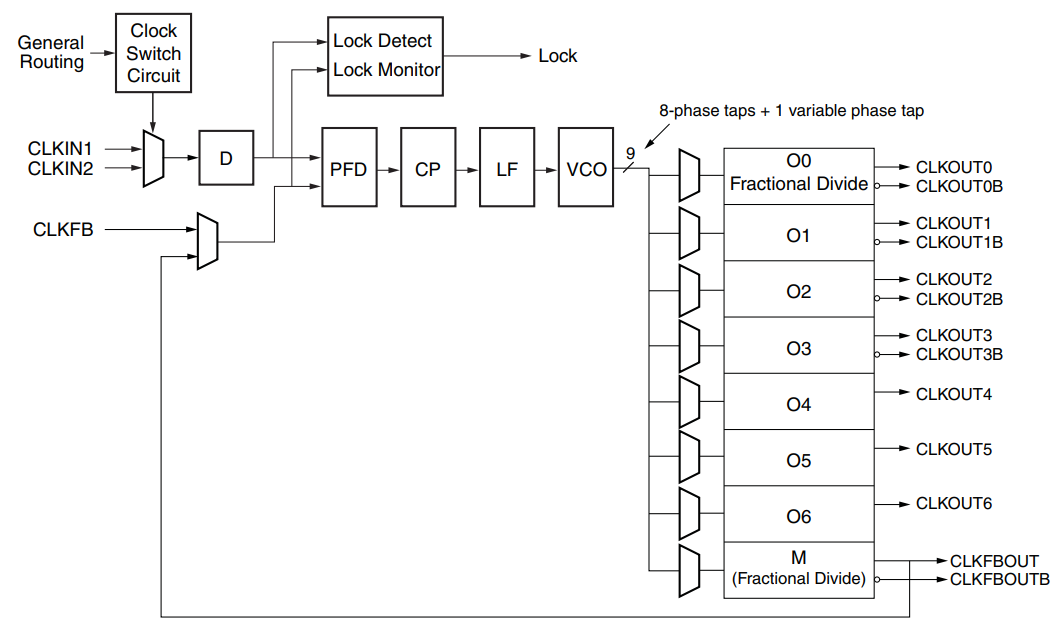
\includegraphics[width=0.5\textwidth]{image/MMCM2_BASE.PNG}
	\caption{Структурная схема примитива MMCM}
	\label{MMCM2_BASE}
\end{figure}

Для того чтобы настроить примитив MMCM необходима следующая информация:

\begin{enumerate}
	\item Частота входного сигнала;
	\item Частоты выходных сигналов(максимум 7);
	\item Коэффициент заполнения выходного сигнала(по умолчанию 50%);
	\item Сдвиг фазы выходных сигналов в градусах относительно фазы входного тактового сигнала;
	\item Полоса пропускания MMCM(по умолчанию установлено значение "OPTIMIZED"), применяется в режиме уменьшения дрожжания("jitter") входного тактового сигнала;
	\item Джиттер("jitter") входного тактового сигнала.
\end{enumerate}

Каждый пункт из списка выше задаётся в виде параметров, назначение, тип данных и диапазон приминимаемых значений которых представлен ниже:

\begin{enumerate}
	\item \verb|BANDWIDTH| определяет алгоритм программирования MMCM, влияющий на джиттер и другие характеристики MMCM. Имеет строковый тип данных и ринимает значения HIGH, LOW, OPTIMIZED.		
	\item \verb|CLKOUT[1:6]_DIVIDE|	 
	определяет величину выходного делителя(обозначен буквой O на структурной схеме) 
	тактовой частоты сигналов CLKOUT[1], CLKOUT[2], CLKOUT[3], CLKOUT[4], CLKOUT[5], CLKOUT[6]. 
	Целое число в диапазоне значений от 1 до 128.
	\item \verb|CLKOUT[0]_DIVIDE_F| определяет величину выходного делителя(обзначен буквой O на структурной схеме) тактовой частоты сигналов CLKOUT[0]. Действительное число в диапазоне значений от 2,000 до 128,000 с шагом 0,125. 	
	\item \verb|CLKOUT[0:6]_PHASE| определяет начальную фазу соответствующего выхода тактового сигнала CLKOUT в смещении в градусах(то есть 90 указывает на сдвиг фазы на 90°). Действительное число в диапазоне от –360.000 до 360.000 in
с шагом 1/56 от FVCO или другим инкрементом, который зависит от \verb|CLKOUT_DIVIDE|.
	\item \verb|CLKOUT[0:6]_DUTY_CYCLE| определяет коэффициент заполнения тактовый сигнала CLKOUT в процентах (то есть 0,50 будет генерировать коэффициент заполнения равный 50\%. Действительное число в диапазоне от 0.01 до 0.99. 
	\item \verb|CLKFBOUT_MULT_F| определяет величину умножения всех выходов тактовых сигналов CLKOUT, если требуется другая частота. Целое число в диапазоне от 2 до 64 или действительное число в диапазоне от 2.000 до 64.000 с инкрементом равным 0.125. 
	\item \verb|DIVCLK_DIVIDE| определяет коэффициент деления для всех выходных тактовых частот по отношению к входной тактовой частоте. Целое число в диапазоне значений от 1 до 106.	
	\item \verb|CLKFBOUT_PHASE| определяет сдвиг фазы в градусах на выходе обратной связи тактового генератора. Сдвиг сигнала обратной связи приводит к отрицательному фазовому сдвигу всех выходных тактовых сигналов на MMCM. Действительное число в диапазоне от 0,00 до 360,00.
	\item \verb|REF_JITTER1| определяет дрожание("jitter") входного тактового сигнала. Действительное число в диапазоне от 0,00 до 0,999.
	Необходим только для моделирования.
	\item \verb|CLKIN1_PERIOD| указывает период входной тактового сигнала в нс для входа MMCM CLKIN1. Разрешение в ps. Эта информация является обязательной и должна быть предоставлена. Действительное число в диапазоне от 0,938 до 100,000. 		
	\item \verb|CLKIN2_PERIOD| указывает период входной тактового сигнала в нс для входа MMCM CLKIN2. Разрешение в ps. Эта информация является обязательной и должна быть предоставлена. Действительное число в диапазоне от 0,938 до 100,000.	
\end{enumerate}

Назначение портов ввода/вывода примитива \(MMCM2_BASE\):

\begin{enumerate}
	\item \verb|CLKIN1(input)| - входной тактовый сигнал №1. 
	\item \verb|CLKIN2(input)| - входной тактовый сигнал №2.
	\item \verb|CLKFBIN(input)| - тактовый сигнал обратной связи.
	\item \verb|CLKINSEL(input)| - управляющий вход мультиплексора выбора входного сигнала: высокий логический уровень \verb|CLKIN1|, 
	низкий логический уровень \verb|CLKIN2|. 
	\item \verb|RST(input)| - асинхронный сигнал сброс.
	\item \verb|PWRDWN(input)| - отключает созданные, но в настоящее время неиспользуемые модули MMCM/PLL. Этот режим можно использовать для экономии энергии для временно неактивных частей схемы и/или MMCM, которые не активны в определенных конфигурациях системы. В этом режиме мощность MMCM/PLL не потребляется. Подайте логическую единицу для отключения MMCM. 
	\item \verb|CLKOUT[0:6](output)| - выходные тактовые сигналы.
	\item \verb|CLKOUT[0:3]B(output)| - инвертированный CLKOUT[0:3].
	\item \verb|CLKFBOUT(output)| - выход обратной связи MMCM.
	\item \verb|CLKFBOUTB(output)| инвертированный выход обратной связи MMCM.
	\item \verb|LOCKED(output)| - выходной сигнал модуля MMCM принимающий значение логической единицы, когда модуль MMCM достиг фазового совмещения в предопределенном окне и согласования частот в предопределенном диапазоне PPM. MMCM автоматически блокируется после включения питания. Дополнительный сброс не требуется. LOCKED принимает значение логического нуля в течение одного тактового цикла частоты фазового детектора, если тактовая частота на входе остановится, будет нарушена синхронизация фаз (например, фазовый сдвиг тактовой частоты на входе) или изменится частота. MMCM должен быть сброшен при снятии подтверждения LOCKED. Тактовые выходы не должны использоваться до утверждения LOCKED.
\end{enumerate}

Рассчитать значение выходной тактовой частоты и значение частоты генератора управляемого напряжением можно по формулам:

\begin{equation}	
	F_{OUT} =  F_{CLKIN} * \frac{M}{D*O},
\end{equation}

\begin{equation}	
	F_{VCO} =  F_{CLKIN} * \frac{M}{D},
\end{equation}

\begin{equation}	
	F_{PFD} =  \frac{F_{CLKIN}}{D} = \frac{F_{VCO}}{M},
\end{equation}

где \textit{M} - \verb|CLKFBOUT_MULT_F|, \textit{O} - \verb|CLKOUT[1:6]_DIVIDE| или \verb|CLKOUT[0]_DIVIDE_F|, \textit{D} - \verb|DIVCLK_DIVIDE|. 	 
При этом заметим, что \(F_{VCO}\) должно лежать в диапазоне от 600 МГц до 1440 МГц, а частота фазового детектора \(F_{PFD}\) должна лежать в диапазоне от 10 МГц до 500 МГц. Частота входного
тактового сигнала \(F_{CLKIN}\) должна лежать в диапазоне от 10 МГц до 933 МГц. Все параметры указаны для ПЛИС установленной на отладочной плате VC707.  

Рассчитаем значение делителей MMCM для \(F_{CLKIN}\) = 200 МГц, а \(F_{OUT}\) = 25 МГц. Пусть \(F_{VCO}\) = 1000 МГц, тогда:

\begin{equation}	
	 \frac{M}{D}  =  \frac{F_{VCO}}{F_{CLKIN}} = 1000/200 = 5,
\end{equation}

тогда примем значения для M = 5, а для D = 1.

\begin{equation}	
	O =  F_{CLKIN} * \frac{M}{D*F_{OUT}} = 200 * 5 / 25 = 40.
\end{equation}

\begin{figure}[!ht]
	\centering
	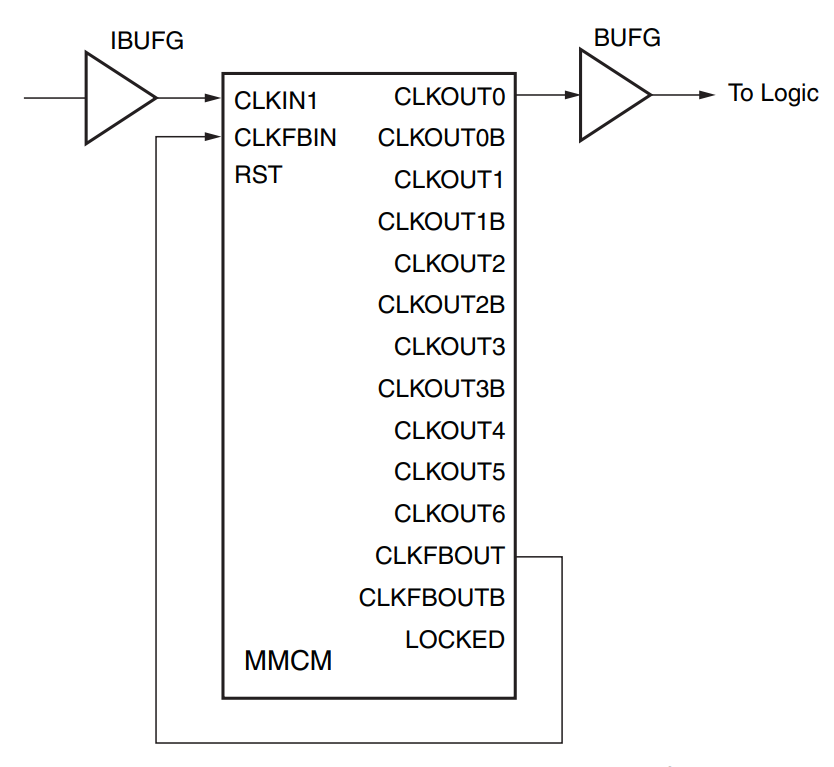
\includegraphics[width=0.5\textwidth]{image/MMCM_INT.PNG}
	\caption{Схема подключения примитива MMCM с внутренней обратной связью}
	\label{fig::MMCM_INT}
\end{figure}

Перейдём к режим работы MMCM. Всего существует два режима работы MMCM: с внутренней и внешней обратной связью. Использование внешней обратной связи нужно если необходимо синхронизация фазы выходных тактовых сигналов со входным. Использование внутренней обратной связи возможно в том случае, если MMCM используется в качестве синтезатора частот или фильтра фазового дрожания, и нет требуемого соотношения фаз между входным тактовым сигналом MMCM и выходным тактовым сигналом MMCM. Производительность MMCM увеличивается, потому что тактовая частота обратной связи не подвержена шуму от источника питания ядра, поскольку он никогда не проходит через блок, питаемый от этого источника. Конечно, шум, вносимый в сигнал CLKIN и BUFG, все равно будет присутствовать. Будем использовать режим с внутренней обратной связью, так как нам не требуется синхронизация фаз входного и выходных тактовых сигналов. На рисунке~\ref{fig::MMCM_INT} представлена схема подключения примитива MMCM с внутренней обратной связью. 

Кроме того, заметим, что входной тактовый сигнал поступает на ПЛИС по дифференциальной паре \verb|clk_in_p|, \verb|clk_in_n|, поэтому для подключения его к примитиву MMCM подребуеться использовать буфер  IBUFGDS, который преобразует дифференциальный тактовый сигнал в обычный("Single-ended")

Обратимся к Vivado Design Suite 7 Series FPGA Libraries Guide для получения Verilog кода подключения \verb|MMCM2_BASE| в наш проект:

\begin{Verbatim}[tabsize=4]
MMCME2_BASE #(
	.BANDWIDTH("OPTIMIZED"),
	.CLKFBOUT_MULT_F(5.0),
	.CLKFBOUT_PHASE(0.0), 
	.CLKIN1_PERIOD(0.0),
	.CLKOUT1_DIVIDE(1),
	.CLKOUT2_DIVIDE(1),
	.CLKOUT3_DIVIDE(1),
	.CLKOUT4_DIVIDE(1),
	.CLKOUT5_DIVIDE(1),
	.CLKOUT6_DIVIDE(1),
	.CLKOUT0_DIVIDE_F(1.0),
	.CLKOUT0_DUTY_CYCLE(0.5),
	.CLKOUT1_DUTY_CYCLE(0.5),
	.CLKOUT2_DUTY_CYCLE(0.5),
	.CLKOUT3_DUTY_CYCLE(0.5),
	.CLKOUT4_DUTY_CYCLE(0.5),
	.CLKOUT5_DUTY_CYCLE(0.5),
	.CLKOUT6_DUTY_CYCLE(0.5),
	.CLKOUT0_PHASE(0.0),
	.CLKOUT1_PHASE(0.0),
	.CLKOUT2_PHASE(0.0),
	.CLKOUT3_PHASE(0.0),
	.CLKOUT4_PHASE(0.0),
	.CLKOUT5_PHASE(0.0),
	.CLKOUT6_PHASE(0.0),
	.CLKOUT4_CASCADE("FALSE"),
	.DIVCLK_DIVIDE(1), 
	.REF_JITTER1(0.0),
	.STARTUP_WAIT("FALSE")
)
MMCME2_BASE_inst (
	.CLKOUT0(CLKOUT0), 
	.CLKOUT0B(CLKOUT0B), 
	.CLKOUT1(CLKOUT1),
	.CLKOUT1B(CLKOUT1B), 	
	.CLKOUT2(CLKOUT2), 		
	.CLKOUT2B(CLKOUT2B), 	
	.CLKOUT3(CLKOUT3), 		
	.CLKOUT3B(CLKOUT3B), 	
	.CLKOUT4(CLKOUT4), 
	.CLKOUT5(CLKOUT5), 
	.CLKOUT6(CLKOUT6), 
	.CLKFBOUT(CLKFBOUT), 
	.CLKFBOUTB(CLKFBOUTB), 
	.LOCKED(LOCKED), 
	.CLKIN1(CLKIN1), 
	.PWRDWN(PWRDWN), 
	.RST(RST), 
	.CLKFBIN(CLKFBIN)
);

\end{Verbatim}

В результате получим следующий код для входного модуля и подключения в нём примитива MMCM:

\begin{Verbatim}[tabsize=4]
`timescale 1ns/1ps

module top_pwm(
    // Clock
    input wire rst,
    // input clk
    input wire clk_in_p,           
    input wire clk_in_n,
    // leds
    output wire led,
    // PWM Fan controller
    output wire pwm
);

// Clock and reset
wire clk_200mhz_ibufg;

// Internal 50 MHz clock
wire clk_mmcm_out;
wire clk_int;
wire rst_int;

wire mmcm_rst = rst;
wire mmcm_locked;
wire mmcm_clkfb;

IBUFGDS
clk_200mhz_ibufgds_inst(
    .I(clk_in_p),
    .IB(clk_in_n),
    .O(clk_200mhz_ibufg)
);

// MMCM instance
// 200 MHz in, 25 MHz out
// M = 5, D = 1 sets Fvco = 1000 MHz (in range)
// Divide by 40 to get output frequency of 25 MHz
MMCME2_BASE #(
    .BANDWIDTH("OPTIMIZED"),
    .CLKOUT0_DIVIDE_F(40),
    .CLKOUT0_DUTY_CYCLE(0.5),
    .CLKOUT0_PHASE(0),
    .CLKOUT1_DIVIDE(8),
    .CLKOUT1_DUTY_CYCLE(0.5),
    .CLKOUT1_PHASE(0),
    .CLKOUT2_DIVIDE(1),
    .CLKOUT2_DUTY_CYCLE(0.5),
    .CLKOUT2_PHASE(0),
    .CLKOUT3_DIVIDE(1),
    .CLKOUT3_DUTY_CYCLE(0.5),
    .CLKOUT3_PHASE(0),
    .CLKOUT4_DIVIDE(1),
    .CLKOUT4_DUTY_CYCLE(0.5),
    .CLKOUT4_PHASE(0),
    .CLKOUT5_DIVIDE(1),
    .CLKOUT5_DUTY_CYCLE(0.5),
    .CLKOUT5_PHASE(0),
    .CLKOUT6_DIVIDE(1),
    .CLKOUT6_DUTY_CYCLE(0.5),
    .CLKOUT6_PHASE(0),
    .CLKFBOUT_MULT_F(5),
    .CLKFBOUT_PHASE(0),
    .DIVCLK_DIVIDE(1),
    .REF_JITTER1(0.010),
    .CLKIN1_PERIOD(5.0),
    .STARTUP_WAIT("FALSE"),
    .CLKOUT4_CASCADE("FALSE")
)
clk_mmcm_inst (
    .CLKIN1(clk_200mhz_ibufg),
    .CLKFBIN(mmcm_clkfb),
    .RST(mmcm_rst),
    .PWRDWN(1'b0),
    .CLKOUT0(clk_mmcm_out),
    .CLKOUT0B(),
    .CLKOUT1(),
    .CLKOUT1B(),
    .CLKOUT2(),
    .CLKOUT2B(),
    .CLKOUT3(),
    .CLKOUT3B(),
    .CLKOUT4(),
    .CLKOUT5(),
    .CLKOUT6(),
    .CLKFBOUT(mmcm_clkfb),
    .CLKFBOUTB(),
    .LOCKED(mmcm_locked)
);

BUFG
clk_bufg_inst (
    .I(clk_mmcm_out),
    .O(clk_int)
);

assign rst_int = ~mmcm_locked;
\end{Verbatim}

Перейдём к разработе ШИМ-контраллера скорости вентилятора. Пусть частота ШИМ-сигнала у нас будет равна 10 кГц. Для получения сигнала с такой частотой напишем счётчик, который поделит наш входной тактовый сигнал частотой равной 25 МГц на величину равную 2500. Код счётчика представлен ниже.

\begin{Verbatim}[tabsize=4]

`timescale 1ns / 1ps

module pwm (
    input clk,
    input rst,
    output pwm
);

reg [15:0] counter_r;

always @(posedge clk) begin 
    if(rst) begin
        counter_r <= 16'b0;
    end else if(counter_r == 'd2499) begin
        counter_r <= 16'b0;
    end else begin
        counter_r <= counter_r + 1;
    end
end

endmodule 

\end{Verbatim}

Для получения широтно-импульсной модуляции введём параметер d. Используя оператор непрервыного присваивания подключим выход \verb|pwm| к компаратору. Теперь при изменении параметра d в диапазоне от 0 до 2500 коэффициент заполнения ШИМ-сигнала будет изменятся в диапазоне от 0 \% до 100 \%. Код ШИМ-контроллера предствлен ниже.

\begin{Verbatim}[tabsize=4]

`timescale 1ns / 1ps

module pwm (
    input clk,
    input rst,
    output pwm
);

reg [15:0] counter_r;

parameter integer d = 1250; 

assign pwm = (d > counter_r) ? 1 : 0; 

always @(posedge clk) begin 
    if(rst) begin
        counter_r <= 16'b0;
    end else if(counter_r == 'd2499) begin
        counter_r <= 16'b0;
    end else begin
        counter_r <= counter_r + 1;
    end
end

endmodule 

\end{Verbatim}

В итоге получаем следующий код, реализующий ШИМ-контроллер:

\begin{Verbatim}[tabsize=4]
`timescale 1ns/1ps

module top_pwm(
    input wire rst,
    // input clk
    input wire clk_in_p,           
    input wire clk_in_n,
    // leds
    output wire led,
    // PWM Fan controller
    output wire pwm
);

// Clock and reset
wire clk_200mhz_ibufg;

// Internal 50 MHz clock
wire clk_mmcm_out;
wire clk_int;
wire rst_int;

wire mmcm_rst = rst;
wire mmcm_locked;
wire mmcm_clkfb;

IBUFGDS
clk_200mhz_ibufgds_inst(
    .I(clk_in_p),
    .IB(clk_in_n),
    .O(clk_200mhz_ibufg)
);

// MMCM instance
// 200 MHz in, 25 MHz out
// M = 5, D = 1 sets Fvco = 1000 MHz (in range)
// Divide by 40 to get output frequency of 25 MHz
MMCME2_BASE #(
    .BANDWIDTH("OPTIMIZED"),
    .CLKOUT0_DIVIDE_F(40),
    .CLKOUT0_DUTY_CYCLE(0.5),
    .CLKOUT0_PHASE(0),
    .CLKOUT1_DIVIDE(8),
    .CLKOUT1_DUTY_CYCLE(0.5),
    .CLKOUT1_PHASE(0),
    .CLKOUT2_DIVIDE(1),
    .CLKOUT2_DUTY_CYCLE(0.5),
    .CLKOUT2_PHASE(0),
    .CLKOUT3_DIVIDE(1),
    .CLKOUT3_DUTY_CYCLE(0.5),
    .CLKOUT3_PHASE(0),
    .CLKOUT4_DIVIDE(1),
    .CLKOUT4_DUTY_CYCLE(0.5),
    .CLKOUT4_PHASE(0),
    .CLKOUT5_DIVIDE(1),
    .CLKOUT5_DUTY_CYCLE(0.5),
    .CLKOUT5_PHASE(0),
    .CLKOUT6_DIVIDE(1),
    .CLKOUT6_DUTY_CYCLE(0.5),
    .CLKOUT6_PHASE(0),
    .CLKFBOUT_MULT_F(5),
    .CLKFBOUT_PHASE(0),
    .DIVCLK_DIVIDE(1),
    .REF_JITTER1(0.010),
    .CLKIN1_PERIOD(5.0),
    .STARTUP_WAIT("FALSE"),
    .CLKOUT4_CASCADE("FALSE")
)
clk_mmcm_inst (
    .CLKIN1(clk_200mhz_ibufg),
    .CLKFBIN(mmcm_clkfb),
    .RST(mmcm_rst),
    .PWRDWN(1'b0),
    .CLKOUT0(clk_mmcm_out),
    .CLKOUT0B(),
    .CLKOUT1(),
    .CLKOUT1B(),
    .CLKOUT2(),
    .CLKOUT2B(),
    .CLKOUT3(),
    .CLKOUT3B(),
    .CLKOUT4(),
    .CLKOUT5(),
    .CLKOUT6(),
    .CLKFBOUT(mmcm_clkfb),
    .CLKFBOUTB(),
    .LOCKED(mmcm_locked)
);

BUFG
clk_bufg_inst (
    .I(clk_mmcm_out),
    .O(clk_int)
);

assign rst_int = ~mmcm_locked;

reg led_r;

assign led = led_r;

always @(posedge clk_int) begin : proc_led
    if(rst_int) begin
        led_r <= 0;
    end else beginB
        led_r <= 1'b1;
    end
end

pwm
pwm_inst 
(
    .clk(clk_int),
    .rst(rst_int),
    .pwm(pwm)
);

endmodule : top_pwm
\end{Verbatim}

Напишем тестбенч для моделирования схемы:

\begin{Verbatim}[tabsize=4]
`timescale 1ns/1ps

module pwm_tb();

    reg sys_clk;
    reg sys_rst;

    initial 
        sys_clk = 1'b0;
    always 
        sys_clk = #(20) ~sys_clk;

    initial begin
        sys_rst = 1'b1;
        #20000
        sys_rst = 1'b0;
    end

    pwm
    pwm_inst
    (
        .clk(sys_clk),
        .rst(sys_rst),
        .pwm()
    );

endmodule
\end{Verbatim}

Напишем файл ограничений для нашего проекта. В этом файле обязательно нужно указать подключение порта светодиода, 
подключение дифференциальной пары тактового сигнала, а также указать величину частоты 
тактового сигнала для временного анализа в Vivado, с помощью команды \verb|create_clock|. Полученный код файла ограничений 
предаставлен ниже. 

\begin{Verbatim}[tabsize=4]
set_property PACKAGE_PIN E19 [get_ports clk_in_p]
set_property IOSTANDARD LVDS [get_ports clk_in_p]
set_property PACKAGE_PIN E18 [get_ports clk_in_n]
set_property IOSTANDARD LVDS [get_ports clk_in_n]

set_property PACKAGE_PIN AV40 [get_ports rst]
set_property IOSTANDARD LVCMOS18 [get_ports rst]

set_property PACKAGE_PIN AM39 [get_ports led]
set_property IOSTANDARD LVCMOS18 [get_ports led]

set_property PACKAGE_PIN BA37 [get_ports pwm]
set_property IOSTANDARD LVCMOS18 [get_ports pwm]

create_clock 	-period 5.000 
				-name sys_clk 
			  	-waveform {0.000 2.500} [get_ports clk_in_p]
\end{Verbatim}

\newpage

Задание:

\begin{enumerate}
	\item
	\item 
	\item 
	\item 
\end{enumerate}